\documentclass[12pt,a4paper]{report}


\usepackage[utf8]{inputenc}
\usepackage[T1]{fontenc}
\usepackage{amsmath}
\usepackage{amsfonts}
\usepackage{amssymb}
\usepackage[francais]{babel}
\usepackage{graphicx}
\usepackage{wrapfig}
\usepackage{hyperref}


\author{Baptiste Rouger}
\title{Rapport de stage}
\date{\today}



\begin{document}

	\begin{titlepage}
		
		\begin{center}
			\vfill
			
			{\Huge \textbf{Rapport de stage}}
			
			\vfill
			
			{\LARGE Baptiste \bsc{Rouger}}
			
			\vfill
			
			{\Huge Analyse de la variation de la taille des plantes lors d'une expérience de sélection divergente pour la date de floraison sur le maïs}
			
			\vfill
			
			{\large\today}
			
			\vfill
			\end{center}
			
			\begin{wrapfigure}[5]{l}[12pt]{5cm}
				
\includegraphics[width=5cm]{logo.jpg}
			\end{wrapfigure} ~\\ %~\\
			UMR de Génétique Quantitative et Evolution - Le Moulon\\
			Ferme du Moulon\\
			91190 Gif-sur-Yvette \\ \\
			
			\begin{figure}[h]
				\centering
				
\includegraphics[width = 4 cm]{inra.jpg}
				
\includegraphics[width = 4 cm]{upsud.jpg}
			\end{figure}
			
			\paragraph*{Directeur de recherche : Olivier \bsc{Martin} \\
			Maître de stage : Christine \bsc{Dillmann}\\
			Enseignant référent : Marianne \bsc{Delarue} }
			\vfill
%		\newpage
	\end{titlepage}
	
	\tableofcontents
	\listoffigures
	\newpage
	
	\section*{Glossaire}
	\addcontentsline{toc}{chapter}{Glossaire}
		\begin{description}
			
			\item [Degré-jour :] mesure utilisée pour calculer l'accumulation de chaleur nécessaire à la durée d'un développement biologique comme la croissance d'une plante
			
			\item [Dérive génétique :] réduction du nombre de génotypes dans une population du fait de phénomènes aléatoires et imprévisibles tels que la rencontre des gamètes
			
			\item [Monoïque :] se dit d'une plante dont les fleurs mâles et femelles sont distinctes mais situées sur le même pied
			
			\item [Sélection naturelle :] mécanisme évolutif issu de la meilleure aptitude de certains individus à la reproduction et la survie que d'autres pour un environnement donné, entraînant la plus grande dispersion de leur génotype
			
		
			
		\end{description}
		 
	
	\chapter{Introduction}
		% faire quelques phrases de présentation ?
		\section{Histoire et généralités du modèle}
			\subsection{Généralités sur le maïs}
				Le maïs (\textit{Zea mays}) est une plante herbacée annuelle appartenant à la famille des \emph{Poacées} (graminées). Par ailleurs, il s'agit d'une plante monoïque.
%				\begin{figure}[!h]
%					\centering
%					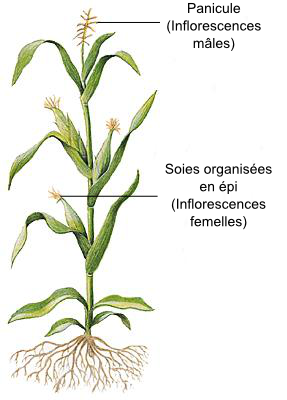
\includegraphics[width=6cm]{monoique.png}
%					\caption{Répartition des organes reproducteurs du maïs}
%					\label{Répartition des organes reproducteurs du maïs}
%				\end{figure}
				\subsubsection{Cycle de vie du maïs}
				Le cycle de vie du maïs commence par la phase de dormance du grain, puis sa germination. Vient ensuite le stade végétatif jeune durant lequel la plante développe ses feuilles juvéniles. Il s'achève par la transition florale qui marque le début du stade végétatif adulte. Celui-ci se termine par la floraison débutant le stade reproducteur. Pour finir, lorsque les graines sont mûres, celles-ci peuvent être récoltées. \cite{tenaillon2}
				\begin{figure}[!h]
					\centering
					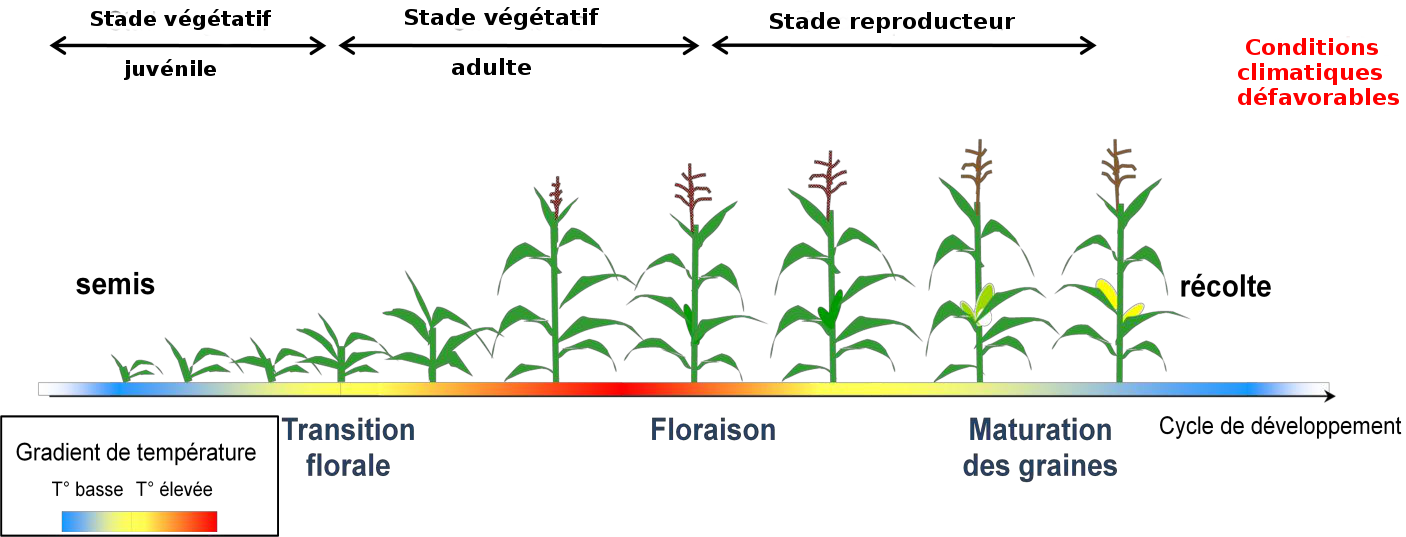
\includegraphics[width=13.7cm]{cycle.png}
					\caption{Cycle de vie du maïs en culture}
					\label{Cycle de vie du maïs en culture}
				\end{figure}
					
			
			\subsection{Histoire du maïs}
				Le maïs est une espèce domestiquée depuis environ 9000 ans. Elle est originaire des alentours de Mexico et est issue de la téosinte (\textit{Zea sp}). Elle s'est rapidement propagée à travers le continent américain\cite{tenaillon} en quelques milliers d'années\footnote{Tenaillon et Charcosset 2011}. Cette expansion demanda son adaptation à des climats plus tempérés que son environnement naturel tropical, ce qui fut réalisé en sélectionnant les variétés insensibles à la photopériode, relativement précoces et capables d'effectuer leur cycle de croissance avant l'arrivée des conditions climatiques défavorable\footnote{\bsc{Figure}~\ref{Cycle de vie du maïs en culture}}. Elle fut découverte et ramenée en Europe par Christophe Colomb lors de sa découverte de l'Amérique, puis disséminée à travers le monde pour devenir la première céréale cultivée.
				\begin{wrapfigure}[9]{r}[12pt]{6.6cm}
					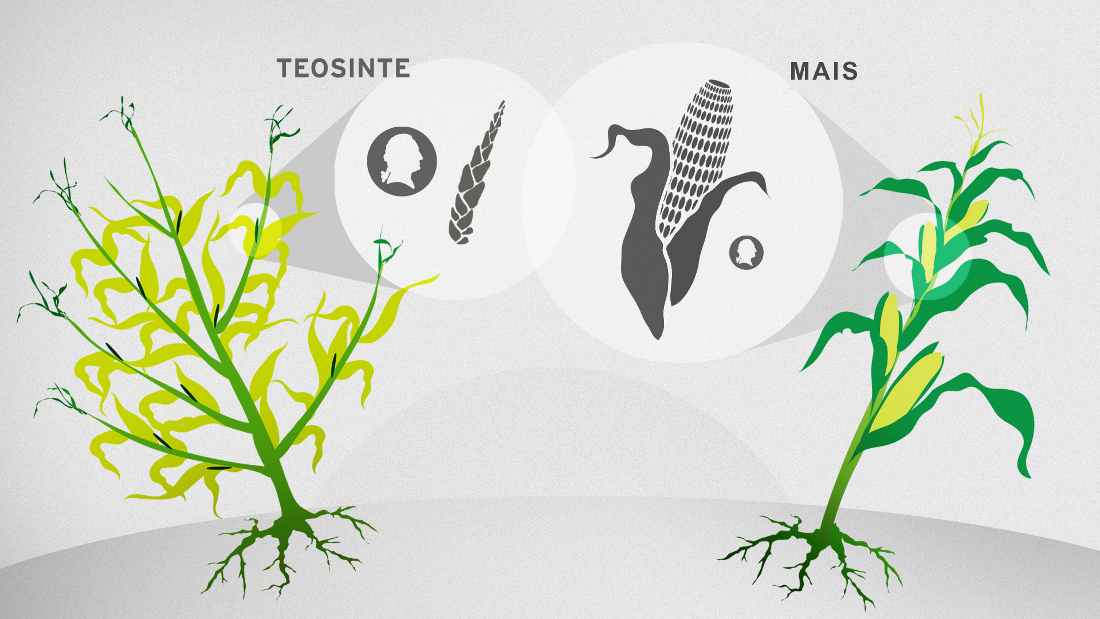
\includegraphics[width=6.6cm]{comparaison.jpg}
					\caption{Comparaison entre téosinte et maïs}
					\label{Comparaison entre téosinte et maïs}
				\end{wrapfigure}
				On remarque également que le maïs possède à présent des caractères dus à sa domestication comme l'absence de dissémination des graines, l'augmentation en nombre et en poids de ces dernières, la synchronisation des dates de floraison des organes mâles et femelles de la plante et une augmentation de la dominance apicale induisant un changement radical de l'architecture de la plante.
				
		\section{Présentation de l'expérimentation}
		
			\subsection{Généralités}
				
				%parler des degrés jour pour la mesure des durées pour les plantes.
				\subsubsection{Des forces évolutives}
				
					Dans une population, présente dans un environnement, les individus interagissent de façon dynamique avec leur environnement. Ces interactions rendent ce système population-environnement dynamique et en évolution permanente. On peut donc observer, au cours du temps, une évolution de la diversité des génotypes, phénotypes, ainsi que des variations de la diversité génétique. On peut alors caractériser les forces qui influent sur la population, comme la dérive génétique, les mutations, la migration des individus, la sélection naturelle... % %manque
					
				\paragraph{L'adaptation}
				
					Il s'agit d'un phénomène résultant des forces évolutives, telle que la sélection. Elle témoigne de la plus grande capacité des individus adaptés à survivre dans leur environnement et à s'y reproduire.
			
			\subsection{L'expérience de sélection divergente}
			
				L'expérience de sélection divergente a débuté en 1993. Prenant pour origine deux lignées pures de maïs (F252 et MBS847) à très forte homozygotie, les plans les plus précoces et les plus tardifs pour la date de floraison furent sélectionnés pour le semis chaque année. On obtient ainsi deux populations de maïs pour une même lignée pure, marquants une plus ou moins forte réponse à la sélection selon la variété et la direction de la sélection (\bsc{Figure}~\ref{sélection}).
				\begin{figure}
					\centering
					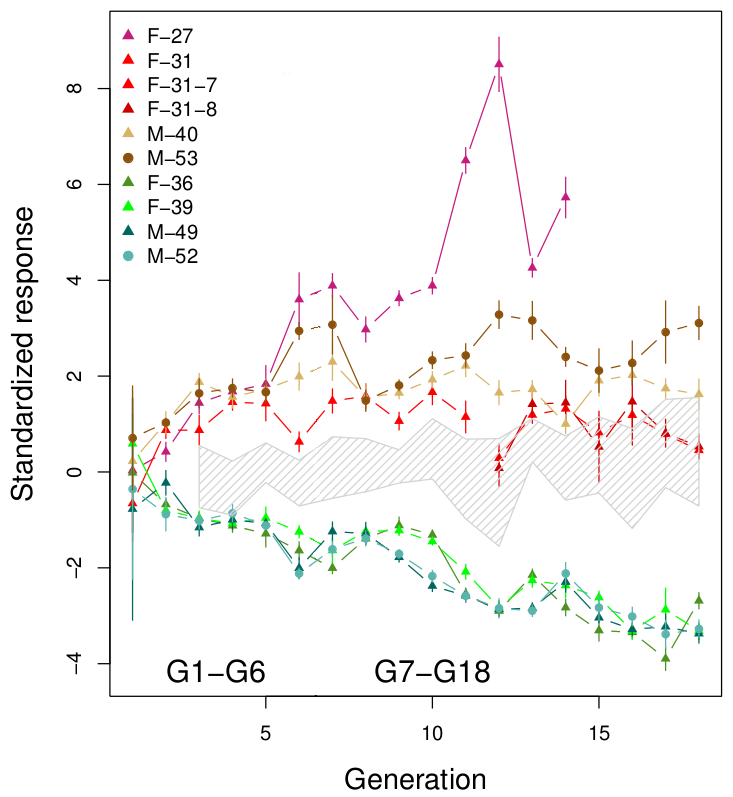
\includegraphics[width = 13.7 cm]{selection.png}
					\caption{Réponse des deux lignées pures de maïs à la sélection pour la date de floraison}
					\label{sélection}
				\end{figure}
				
				Par ailleurs, la taille des maïs fut aussi mesurée, pour observer si, comment, et combien un caractère n'intervenant pas dans la sélection artificielle d'un individu pouvait être modifié par celle-ci.
			
		\section{Objectifs du stage}
		
			Une analyse fine des paramètres de taille pour chaque population de maïs doit être faite pour déterminer dans quelle mesure les plantes voient leur taille varier par la sélection faite sur la date de floraison.
			
	\begin{quotation}
		Après nous êtres intéressés au matériel utilisé lors des vingt années d'expérimentation, nous nous intéresserons au méthodes de traitement des données. Nous analyserons ensuite les résultats et les interpréterons. Enfin, nous conclurons ce sujet.
	\end{quotation}
	
	
	\chapter{Matériel et méthodes}
		
		\section{Le matériel végétal}
			
			L'expérience de sélection divergente (\bsc{Figure}~\ref{selec.div}), débutée en 1993 \textit{VERIFICATION} et toujours en cours, compte 19 générations de maïs. Les souches de départ utilisées sont deux lignées pures à forte homozygotie : les maïs F252 et MBS847 (notée MBS). On obtient alors deux lots de semences séparées de plusieurs semaines pour la date de floraison\footnote{Définie lorsque les fleurs mâles et femelles apparaissent} qui sont notées en degrés-jours.
			
			A chaque génération, on réalise pour chaque lignée une autofécondation\footnote{Pour réaliser l'autofécondation, on couvre les fleurs des individus de sachets pour recueillir le pollen et protéger les soies. Après vingt-quatre heures, le sachet contenant le pollen est déposé sur la fleur femelle pour réaliser l'autofécondation.} des dix individus les plus précoces et les plus tardifs. Pour pouvoir retracer le pedigree de chaque individus semé et sélectionné, on réalise des cartes généalogiques (\bsc{Figure}~\ref{carte_gen}) des lignées de maïs. Les individus sélectionnés à la dernière génération sont indiqués en couleur, ainsi que tous leurs descendants. \cite{goossens93}
			
			\begin{figure}
				\centering
				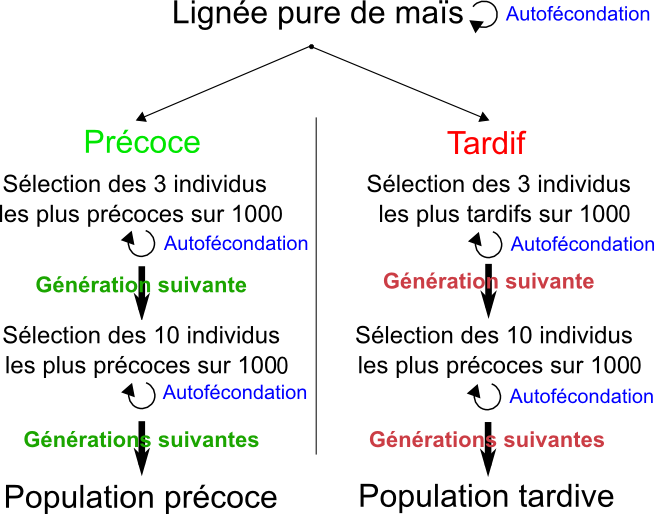
\includegraphics[width=6.5cm]{selec_div.png}
				\caption{Principe de l'expérience de sélection divergente}
				\label{selec.div}
			\end{figure}
			\begin{figure}
				\centering
				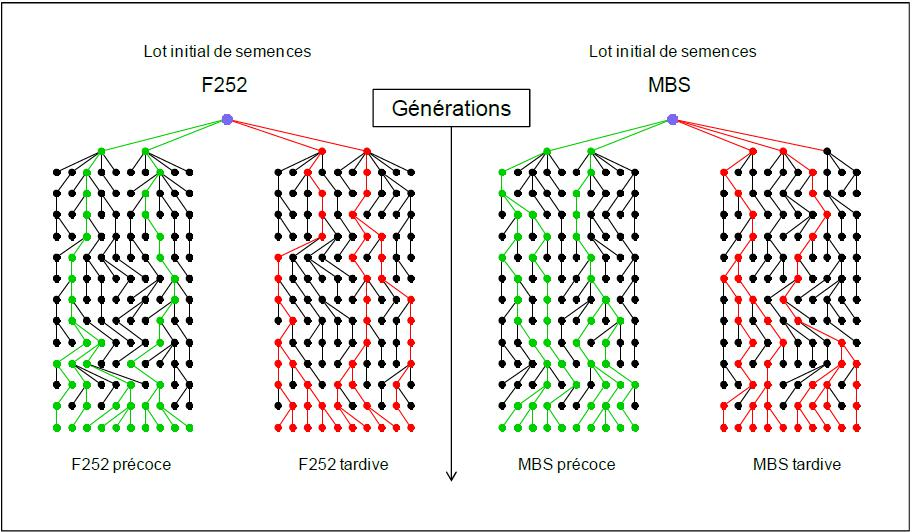
\includegraphics[width = 6.5 cm]{carte_gen.jpg}
				\caption{Carte génétique des deux lignées de maïs F252 et MBS pour l'expérience de sélection divergente en 2012}
				\label{carte_gen}
			\end{figure}
			
		\section{Méthodes}
			
			Pour réaliser les analyses nécessaires à la confirmation de nos hypothèses, il faut commencer par formater toutes les données au même format, c'est à dire que chaque plante mesurée sera référencée avec de nombreuses caractéristiques la concernant : l'année, la génération, la lignée (F252 ou MBS), le parent (c'est-à-dire le \og grand-parent \fg de la plante mesurée), le progéniteur (le parent de la plante), la population à laquelle elle appartient (tardive, précoce ou témoin), la famille qui permet de retracer la généalogie, le bloc, la ligne et le numéro de la plante qui permettent de retrouver la position de la plante dans le champs, et bien évidemment la hauteur de la plante.
			
	\bibliographystyle{plain}
	\bibliography{rapport}
	
	\appendix
	
	\chapter{Codes sources}
	Les codes sources utilisés pendant ce stage sont disponibles sur Github à l'adresse suivante : \url{https://github.com/rougerbaptiste/stageL2}.\\~\\
	Voici la fonction de chacun de ces codes :
	\begin{description}
		\item [aggregate.R :] Ce script a pour fonction de rassembler les données contenues dans les fichiers de hauteurs de chaque année pour les rassembler dans un unique fichier.
		\item [RprFam.R :] Ce script a pour fonction de représenter les données de hauteurs obtenues pour chaque famille (hauteur absolue et hauteur relative au témoin) et de créer un fichier .pdf contenant les deux graphes.
		\item [RprPop.R :] Ce script a pour fonction de représenter les données de hauteurs obtenues pour chaque population (hauteur absolue et hauteur relative au témoin) et de créer un fichier .pdf contenant les deux graphes.
		\item [tri.R :] Ce script a pour fonction de récupérer toutes les données brutes de hauteurs, de les mettre sous une forme standard et de créer un fichier contenant les données de hauteur par année.
		
	\end{description}
\end{document}
